\section{Method}
\label{sec:method}

PICHS links scene-level clearance reasoning to contact-feasible multi-robot
execution. Given a start--goal query for a large vehicle in clutter, PICHS
first tests whether a~$W$-clear corridor already exists. If passage is
blocked, it identifies reachable bottlenecks, generates local pushing
modes only for those bottlenecks, and validates selected interventions
through simulation. The overall pipeline is shown in
Fig.~\ref{fig:overall}.

\subsection{WCCG Representation and Reachable Bottlenecks}
\label{subsec:frontier}

The scene is represented by a~$W$-clearance connectivity graph, abbreviated
WCCG, whose role is to expose the search-relevant clearance structure without
recovering a detailed geometric path at every step. The graph is constructed
directly from obstacle geometry in a width-aware manner. Centroid nodes encode
obstacle components, and bridge relations encode local inter-obstacle
passages. The resulting graph is defined as
$\mathcal{G}_W \triangleq (\mathcal{V}, \mathcal{E}_c \cup \mathcal{E}_b)$,
where~$\mathcal{V}$ contains centroid and bridge nodes,
$\mathcal{E}_c$ denotes centroid--bridge edges, and
$\mathcal{E}_b$ denotes bridge--bridge edges. Each bridge edge is annotated
with a local width~$w_{uv}$, defined by the distance between the associated
closest points on the two neighboring components. This makes~$\mathcal{G}_W$
a compact representation of where the scene is already traversable and where
narrow passages arise. In particular, the WCCG does not attempt to enumerate
all possible obstacle rearrangements. Its role is to expose the small subset
of bottlenecks that currently determines whether a~$W$-clear corridor can be
formed.

Given the vehicle start and goal, a width-constrained connectivity query is
performed on~$\mathcal{G}_W$. If the two lie in the same~$W$-clear connected
face, then a feasible corridor already exists and no clearing action is
needed, i.e.,
\begin{equation}\label{eq:wccg-criterion}
\{\mathbf{s}_{\mathrm{V}}^{\mathrm{S}},\;
\mathbf{s}_{\mathrm{V}}^{\mathrm{G}}\}
\emph{ belong to the same face of } \mathcal{G}_W,
\end{equation}
which states that the start and goal of the large vehicle are already
connected through the same width-feasible free-space region.
If~\eqref{eq:wccg-criterion} does not hold, the query returns the current
reachable frontier loop~$\mathcal{L}$ that separates the two sides under the
width constraint. The bridge--bridge edges visible on~$\mathcal{L}$ define
the first-hop set of reachable bottlenecks,
$\Gamma_{\mathcal{L}} \triangleq \{g_1, \cdots, g_K\}$, where each~$g_k$ is a
candidate gap exposed by the current clearance query.
In PICHS, these frontier gaps are an internal search interface rather than the
primary methodological contribution. Their role is to translate the global
clearance query into a compact local decision set. More precisely, each
$g \in \Gamma_{\mathcal{L}}$ identifies a reachable place where a small
increase in local clearance may change the global connectivity outcome.
Subsequent stages therefore do not generate contact actions over the full
scene. Instead, they operate only on~$\Gamma_{\mathcal{L}}$, which converts
scene-level bottlenecks into compact contact-feasible queries for
multi-robot pushing.

\subsection{Gap-Conditioned Pushing Mode Generation}
\label{subsec:modes}

For a frontier gap~$g \in \Gamma_{\mathcal{L}}$ under consideration, the next
question is whether this reachable bottleneck can be enlarged through
executable multi-robot interaction. The role of this stage is therefore not to
solve a fully general manipulation problem, but to convert a scene-level
clearance bottleneck into a small set of contact-feasible intervention
queries.

Let~$\Omega_m$ denote one of the movable obstacles adjacent to~$g$. For each
such obstacle, a small set of short-horizon obstacle motion intents
$\{\mathbf{v}_m^k\}_{k=1}^{K_m}$ is sampled, where
$\mathbf{v}_m^k \triangleq (v_x, v_y, \omega) \in \mathbb{R}^3$. The sampled
directions are biased toward local gap-opening motions while allowing some
rotational components to account for local geometry. This bias is important.
It steers the candidate set toward motions that are likely to widen the
selected bottleneck, while still preserving enough directional variation to
capture cases in which rotation or oblique contact produces a better opening
effect than pure translation. These sampled directions are the candidate
pushing intents for the obstacles adjacent to~$g$.

For each sampled direction~$\mathbf{v}_m^k$, an associated pushing mode
$\boldsymbol{\xi} \triangleq (\mathcal{C}, \mathbf{u})$ is generated, where
$\mathcal{C}$ denotes the robot--object contact configuration and
$\mathbf{u}$ denotes the associated contact wrench parameters. Let
$\mathbf{v}_m^{k,\mathrm{B}} \in \mathbb{R}^3$ denote~$\mathbf{v}_m^k$
expressed in the body frame of~$\Omega_m$. This body-frame representation
makes the feasibility score depend on the local contact geometry of the object
rather than on the global scene orientation. A pushing mode is evaluated by
the primary and multi-directional feasibility losses
\begin{equation}
\label{eq:mode-feasibility}
\begin{aligned}
\mathrm{J}_{\mathrm{F}}^m
(\boldsymbol{\xi}, \mathbf{v}_m^{k,\mathrm{B}})
&\triangleq
\min_{\mathbf{q}_{m,\boldsymbol{\xi}} \in
\mathrm{Q}_{m,\boldsymbol{\xi}}}
\left\|
\mathbf{q}_{m,\boldsymbol{\xi}} +
Q_\mu^m(\mathbf{v}_m^{k,\mathrm{B}})
\right\|_1, \\
\mathrm{J}_{\mathrm{MF}}^m
(\boldsymbol{\xi}, \mathbf{v}_m^{k,\mathrm{B}})
&\triangleq
\sum_{\mathbf{v}_d \in \mathcal{D}} w_d \cdot
\mathrm{J}_{\mathrm{F}}^m(\boldsymbol{\xi}, \mathbf{v}_d),
\end{aligned}
\end{equation}
where~$\mathbf{q}_{m,\boldsymbol{\xi}} \in \mathbb{R}^3$ is a feasible body
wrench induced by mode~$\boldsymbol{\xi}$,
$\mathrm{Q}_{m,\boldsymbol{\xi}} \subseteq \mathbb{R}^3$ is the corresponding
admissible wrench set under local contact and friction constraints,
$Q_\mu^m(\mathbf{v}_m^{k,\mathrm{B}})$ is the quasi-static friction wrench of
$\Omega_m$ along~$\mathbf{v}_m^{k,\mathrm{B}}$, and~$\mathcal{D}$ with weights
$w_d$ augments the desired direction by neighboring basis velocities.
Similar measures are also adopted
in~\cite{tang2024collaborative,tang2025pushingbots}.
Small~$\mathrm{J}_{\mathrm{F}}^m$ is necessary for force feasibility, whereas
small~$\mathrm{J}_{\mathrm{MF}}^m$ indicates a mode that remains effective
under small directional perturbations.
Accordingly, the associated mode
is obtained by sparse constrained optimization over reachable contacts on
$\partial \Omega_m$ and is defined as
$\boldsymbol{\xi}_m^k \triangleq (\mathcal{C}_m^k, \mathbf{u}_m^k)$. The
optimization minimizes
$\mathrm{J}_{\mathrm{MF}}^m(\boldsymbol{\xi}, \mathbf{v}_m^{k,\mathrm{B}})$
under local friction and wrench constraints. Only the best few pairs
$(\mathbf{v}_m^k, \boldsymbol{\xi}_m^k)$ are retained, while a persistent
\emph{ModeTable} reuses effective entries across similar local geometries.
This reuse reduces repeated contact optimization for geometrically similar
local arrangements and keeps the candidate set compact. Each retained pushing
candidate therefore takes the form~$(g, \mathbf{v}, \boldsymbol{\xi})$, and
the gap-induced candidate set is denoted by~$\Xi_g$.

A candidate pushing mode is retained only if it passes short-horizon physical
validation. The robots must be able to reach the proposed pre-contact poses,
avoid collision during approach and pushing, maintain stable contact, and
induce obstacle motion that actually enlarges the target gap. This validation
is performed by the short-horizon rollout
\begin{equation}
\label{eq:sim}
(\mathbf{s}', \delta_T, \delta_J)
\triangleq
\mathsf{EvalSim}\bigl(\mathbf{s}, (g, \mathbf{v}, \boldsymbol{\xi})\bigr),
\end{equation}
which returns the successor state, time cost, and control effort. The
validation step is important because low analytical feasibility loss alone
does not guarantee executable multi-robot behavior in dense clutter. This
stage therefore does not enumerate contact actions over the full scene.
Instead, it converts each reachable bottleneck into a compact set of
physically testable multi-robot interventions for the search.

\begin{figure}[t!]
  \centering
  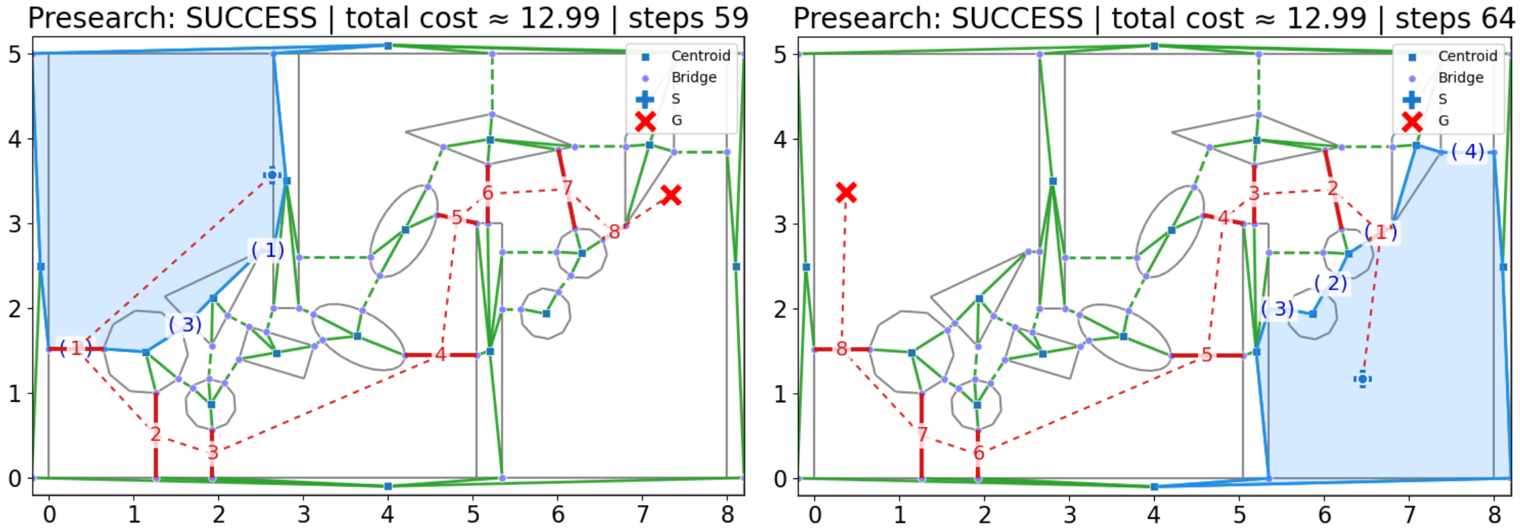
\includegraphics[width=0.98\linewidth]{figures/presearch_1col.png}
  \vspace{-0.15in}
  \caption{
    Ranked reachable bottlenecks under swapped start--goal queries in the same
    scene. Each panel shows the WCCG with the current reachable face in light
    blue. Candidate gaps on the frontier loop are ranked by local priority in
    blue and refined by short presearch in red.
  }
  \label{fig:presearch}
  \vspace{-4mm}
\end{figure}

\subsection{Selective Expansion in PICHS}
\label{subsec:pichs}

At node~$\nu$, PICHS first checks whether the current state satisfies the
connectivity criterion in~\eqref{eq:wccg-criterion}. If not, the updated WCCG
induces a reachable frontier loop~$\mathcal{L}_\nu$ and the associated
candidate gaps~$\Gamma_{\mathcal{L}_\nu}$. As illustrated in
Fig.~\ref{fig:presearch}, these gaps are ranked by the predicted
cost-to-connect
\begin{equation}
\label{eq:gap-score}
\widehat{\mathsf{Cost}}(g)
\triangleq
\mathsf{C}(g \mid \mathcal{L}_\nu, \mathbf{s}_{\mathcal{R}})
+
\mathsf{C}_{\mathrm{pre}}(g),
\end{equation}
where~$\mathsf{C}(g \mid \mathcal{L}_\nu, \mathbf{s}_{\mathcal{R}})$ combines
the robots' transition cost to the gap and the estimated effort required to
widen it, and~$\mathsf{C}_{\mathrm{pre}}(g)$ is a short presearch estimate of
downstream gap-crossing cost toward the goal. The first term therefore
captures how expensive the candidate is to activate from the current state,
whereas the second term estimates whether opening that gap is likely to
improve progress toward a full corridor.
The ranked list is defined by
$\mathsf{Rank}(\nu)
\triangleq
\operatorname{argsort}_{g \in \Gamma_{\mathcal{L}_\nu}}
\widehat{\mathsf{Cost}}(g)$,
and the node priority is defined by
$\label{eq:node-priority}
f(\nu)
\triangleq
\chi(\nu)
+
\min_{g \in \mathsf{Rank}(\nu)} \widehat{\mathsf{Cost}}(g)$,
where~$\chi(\nu)$ is the realized path cost accumulated from the root to node
$\nu$. Equation~\eqref{eq:node-priority} therefore balances what has already
been spent against the best currently predicted remaining cost. This balance
encourages PICHS to prefer nodes that are both physically promising and
globally efficient. Alg.~\ref{alg:pichs} summarizes the resulting selective
expansion loop.

\begin{algorithm}[t!]
\caption{Selective Expansion in PICHS}
\label{alg:pichs}
\SetAlgoLined
\KwIn{$\mathbf{s}_0$,~$\alpha$,~$\mathsf{EvalSim}(\cdot)$}
\KwOut{$\pi^\star$}
$\nu_0 \gets (\mathbf{s}_0, \emptyset),\; \chi(\nu_0) = 0$\;
Initialize~$\mathcal{Q}$ by~\eqref{eq:node-priority}\;
\While{$\mathcal{Q} \neq \emptyset$}{
 $\nu = (\mathbf{s}, \pi) \gets \mathcal{Q}.\texttt{pop\_min}()$\;
  \If{$\mathbf{s}$ satisfies~\eqref{eq:wccg-criterion}}{
   $\pi^\star \gets \pi$, \textbf{break}\;
  }
  Update the WCCG and construct~$\mathsf{Rank}(\nu)$\;
  \ForEach{$g \in \mathsf{Rank}(\nu)$}{
    Generate~$\Xi_g$\;
    \ForEach{$(\mathbf{v}, \boldsymbol{\xi}) \in \Xi_g$}{
     $\tau \triangleq (g, \mathbf{v}, \boldsymbol{\xi})$\;
     $(\mathbf{s}', \delta_T, \delta_J)
      \gets \mathsf{EvalSim}(\mathbf{s}, \tau)$\;
      \If{success}{
       $\nu' \gets (\mathbf{s}', \pi \cup \{\tau\})$\;
       $\chi(\nu') \gets
        \chi(\nu) + \delta_T + \alpha \, \delta_J$\;
       $\mathcal{Q}.\texttt{push}(\nu')$\;
      }
    }
  }
}
\Return{$\pi^\star$}\;
\end{algorithm}

For each ranked gap~$g \in \mathsf{Rank}(\nu)$, PICHS calls the gap-conditioned
mode generator in Sec.~\ref{subsec:modes}. There, constrained mode
generation guided by~\eqref{eq:mode-feasibility} produces a compact
set~$\Xi_g$, and each candidate
$\tau \triangleq (g, \mathbf{v}, \boldsymbol{\xi})$ is evaluated by the
short-horizon rollout in~\eqref{eq:sim}. PICHS is selective in three senses.
The WCCG restricts to reachable bottlenecks. Gap ranking prioritizes
which bottlenecks to test first. Candidate generation together with
short-horizon simulation validates only those interventions worth expanding.
This selectivity is the main reason PICHS remains tractable in dense
clutter. It reduces the branching factor before simulation, and it reserves
physics evaluation for actions that are  relevant to corridor
construction. Repeating this loop yields a clearing schedule that
specifies which gaps to open and how to open them.
